\tikzset{every picture/.style={line width=0.75pt}}
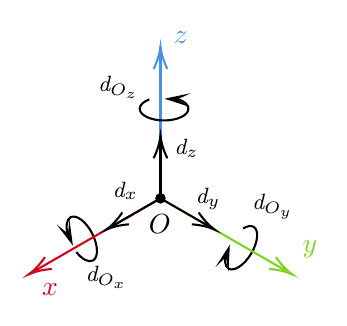
\begin{tikzpicture}[x=0.75pt,y=0.75pt,yscale=-1,xscale=1]
    \draw [color={rgb, 255:red, 74; green, 144; blue, 226 }  ,draw opacity=1 ]   (249.79,80.38) -- (249.79,9.08) ;
    \draw [shift={(249.79,7.08)}, rotate = 90] [color={rgb, 255:red, 74; green, 144; blue, 226 }  ,draw opacity=1 ][line width=0.75]    (10.93,-3.29) .. controls (6.95,-1.4) and (3.31,-0.3) .. (0,0) .. controls (3.31,0.3) and (6.95,1.4) .. (10.93,3.29)   ;
    \draw  [draw opacity=0] (257.99,32.5) .. controls (261.16,33.51) and (263.25,35.24) .. (263.25,37.21) .. controls (263.25,40.32) and (258,42.85) .. (251.52,42.85) .. controls (245.05,42.85) and (239.8,40.32) .. (239.8,37.21) .. controls (239.8,35.38) and (241.61,33.75) .. (244.41,32.72) -- (251.52,37.21) -- cycle ; \draw   (257.99,32.5) .. controls (261.16,33.51) and (263.25,35.24) .. (263.25,37.21) .. controls (263.25,40.32) and (258,42.85) .. (251.52,42.85) .. controls (245.05,42.85) and (239.8,40.32) .. (239.8,37.21) .. controls (239.8,35.38) and (241.61,33.75) .. (244.41,32.72) ;
    \draw  [draw opacity=0] (205.05,97.73) .. controls (204.06,93.79) and (204.55,90.48) .. (206.55,89.46) .. controls (209.33,88.05) and (213.96,91.58) .. (216.9,97.35) .. controls (219.84,103.12) and (219.97,108.94) .. (217.19,110.35) .. controls (215.09,111.42) and (211.93,109.66) .. (209.25,106.25) -- (211.87,99.91) -- cycle ; \draw   (205.05,97.73) .. controls (204.06,93.79) and (204.55,90.48) .. (206.55,89.46) .. controls (209.33,88.05) and (213.96,91.58) .. (216.9,97.35) .. controls (219.84,103.12) and (219.97,108.94) .. (217.19,110.35) .. controls (215.09,111.42) and (211.93,109.66) .. (209.25,106.25) ;
    \draw  [draw opacity=0] (289.6,94.92) .. controls (291.53,93.69) and (293.37,93.33) .. (294.68,94.12) .. controls (297.34,95.72) and (296.8,101.52) .. (293.45,107.07) .. controls (290.11,112.61) and (285.24,115.81) .. (282.57,114.2) .. controls (280.67,113.05) and (280.4,109.78) .. (281.61,105.98) -- (288.62,104.16) -- cycle ; \draw   (289.6,94.92) .. controls (291.53,93.69) and (293.37,93.33) .. (294.68,94.12) .. controls (297.34,95.72) and (296.8,101.52) .. (293.45,107.07) .. controls (290.11,112.61) and (285.24,115.81) .. (282.57,114.2) .. controls (280.67,113.05) and (280.4,109.78) .. (281.61,105.98) ;
    \draw  [fill={rgb, 255:red, 0; green, 0; blue, 0 }  ,fill opacity=1 ] (205.98,94.78) -- (206.86,101.37) -- (202.81,96.09) -- (205.63,98.4) -- cycle ;
    \draw  [fill={rgb, 255:red, 0; green, 0; blue, 0 }  ,fill opacity=1 ] (279.01,110.18) -- (282.61,104.59) -- (282.28,111.23) -- (281.63,107.65) -- cycle ;
    \draw  [fill={rgb, 255:red, 0; green, 0; blue, 0 }  ,fill opacity=1 ] (260,34.53) -- (253.67,32.48) -- (260.18,31.11) -- (256.88,32.65) -- cycle ;
    \draw [color={rgb, 255:red, 126; green, 211; blue, 33 }  ,draw opacity=1 ]   (249.79,80.38) -- (311.53,116.02) ;
    \draw [shift={(313.27,117.02)}, rotate = 210] [color={rgb, 255:red, 126; green, 211; blue, 33 }  ,draw opacity=1 ][line width=0.75]    (10.93,-3.29) .. controls (6.95,-1.4) and (3.31,-0.3) .. (0,0) .. controls (3.31,0.3) and (6.95,1.4) .. (10.93,3.29)   ;
    \draw [color={rgb, 255:red, 208; green, 2; blue, 27 }  ,draw opacity=1 ]   (249.79,80.37) -- (218.61,98.38) -- (188.04,116.02) ;
    \draw [shift={(186.31,117.02)}, rotate = 330] [color={rgb, 255:red, 208; green, 2; blue, 27 }  ,draw opacity=1 ][line width=0.75]    (10.93,-3.29) .. controls (6.95,-1.4) and (3.31,-0.3) .. (0,0) .. controls (3.31,0.3) and (6.95,1.4) .. (10.93,3.29)   ;
    \draw    (249.79,80.38) -- (249.79,52.13) ;
    \draw [shift={(249.79,50.13)}, rotate = 90] [color={rgb, 255:red, 0; green, 0; blue, 0 }  ][line width=0.75]    (10.93,-3.29) .. controls (6.95,-1.4) and (3.31,-0.3) .. (0,0) .. controls (3.31,0.3) and (6.95,1.4) .. (10.93,3.29)   ;
    \draw    (249.79,80.38) -- (274.25,94.5) ;
    \draw [shift={(275.99,95.5)}, rotate = 210] [color={rgb, 255:red, 0; green, 0; blue, 0 }  ][line width=0.75]    (10.93,-3.29) .. controls (6.95,-1.4) and (3.31,-0.3) .. (0,0) .. controls (3.31,0.3) and (6.95,1.4) .. (10.93,3.29)   ;
    \draw    (249.79,80.37) -- (225.32,94.5) ;
    \draw [shift={(223.59,95.5)}, rotate = 330] [color={rgb, 255:red, 0; green, 0; blue, 0 }  ][line width=0.75]    (10.93,-3.29) .. controls (6.95,-1.4) and (3.31,-0.3) .. (0,0) .. controls (3.31,0.3) and (6.95,1.4) .. (10.93,3.29)   ;
    \draw (191.23,119.9) node [anchor=north west][inner sep=0.75pt]  [color={rgb, 255:red, 208; green, 2; blue, 27 }  ,opacity=1 ]  {$x$};
    \draw (316.73,99.4) node [anchor=north west][inner sep=0.75pt]  [color={rgb, 255:red, 126; green, 211; blue, 33 }  ,opacity=1 ]  {$y$};
    \draw (254.73,-1.35) node [anchor=north west][inner sep=0.75pt]  [color={rgb, 255:red, 74; green, 144; blue, 226 }  ,opacity=1 ]  {$z$};
    \draw (212.25,111.65) node [anchor=north west][inner sep=0.75pt]  [font=\footnotesize]  {$\mathit{d}_{O_{x}}$};
    \draw (218.25,20.15) node [anchor=north west][inner sep=0.75pt]  [font=\footnotesize]  {$\mathit{d}_{O_{z}}$};
    \draw (292.5,76.9) node [anchor=north west][inner sep=0.75pt]  [font=\footnotesize]  {$\mathit{d}_{O_{y}}$};
    \draw (255,50.4) node [anchor=north west][inner sep=0.75pt]  [font=\footnotesize]  {$\mathit{d}_{z}$};
    \draw (225.25,70.9) node [anchor=north west][inner sep=0.75pt]  [font=\footnotesize]  {$\mathit{d}_{x}$};
    \draw (265.25,73.9) node [anchor=north west][inner sep=0.75pt]  [font=\footnotesize]  {$\mathit{d}_{y}$};
    \draw (242.75,86.65) node [anchor=north west][inner sep=0.75pt]    {$O$};
    \draw [fill={rgb, 255:red, 0; green, 0; blue, 0 }  ,fill opacity=1 ]  (249.79, 80.38) circle [x radius= 2, y radius= 2]   ;
\end{tikzpicture}